\documentclass[letterpaper]{article}
\usepackage{aaai20}
\usepackage{times}
\usepackage{helvet}
\usepackage{courier}
\usepackage[hyphens]{url} 
\usepackage{graphicx}
\graphicspath{./}
\usepackage{todonotes}
\usepackage[acronym]{glossaries}
\urlstyle{rm}
\def\UrlFont{\rm}
\usepackage{graphicx}
\frenchspacing
\setlength{\pdfpagewidth}{8.5in}
\setlength{\pdfpageheight}{11in}
\pdfinfo{
/Title (Applying CBR Retrieval and Rule-Based Heuristics to Improve Alpha-Beta Search in Chess)
/Author (Josep Han, Rowan Lavelle, Zachary Wilkerson)
}
\title{Applying CBR Retrieval and Rule-Based Heuristics to Improve Alpha-Beta Search in Chess}
\author{Josep Han, Rowan Lavelle, Zachary Wilkerson}
\date{April 2021}

\newacronym{cbr}{CBR}{case-based reasoning}

\begin{document}

\maketitle
\section{Abstract}
\section{Introduction}
\section{Related Work}
\section{Model Overview}

\subsection{Pruning the Search Space}
Since minimax is a search-based algorithm, it naturally follows that a wrapper algorithm that can efficiently prune away parts of the search space from consideration potentially can create a significant performance increase.  We explore a progression of several model concepts, ultimately using a rule-based system to prune the search space using broad playing principles.

\subsubsection{1st Attempt: Case-Based Reasoning}
Intuitively, pruning away unreasonable moves from the search space appears well-suited for a \acrshort{cbr} approach, where a board state is analyzed holistically against a case base, allowing multiple specific prunings to be applied.  For example, it is traditionally unwise to move any of the pawns in front of the king after castling, as this exposes the king to attack.  In this instance, the similarity function is the location of the king (and optionally the positions of the pawns in front of it), and the solution is to prune away moves involving those pawns from consideration.  Now consider an instance where the opponent has moved their queen to a square threatened by one of the pawns.  Assuming this is not an intentional sacrifice, an exception to the case-based rule is required.  These would take the form of adaptations; continuing with the example, if a high-value piece may be captured by one of the pawns, we can override the initial solution and consider the pawn's move.  Feasibly, such a model could apply at a high resolution across diverse scenarios, including threats, pins, sacrifices, etc.

However, the granularity of this model is too much, and the resultant cost for comparing a board state against many cases far outweighs the cost of considering the moves anyway (at least when evaluated at shallow depths like we used for testing).  Furthermore, the amount of knowledge engineering to arrange moves in a rule-exception format is also very high.  This problem necessitates considering positional information from the board in a stricter, rule-based format that requires fewer calculations and reaches more absolute conclusions.

\subsubsection{2nd Attempt: Hierarchy of Rules}
Building on weaknesses of the \acrshort{cbr} approach, the hierarchy of rules sought to limit the moves considered by the player (and pruning the rest).  This process starts with high-level situational rules that then lead into specific responses.  An example situational rule might activate if a piece is threatened; specific responses might be to move the piece (especially if it is threatened by an inferior piece), to support the threatened piece with another and promote an exchange, etc.  This enables a sort of de facto pruning where moves that do not fall within the umbrella of the situational rules are pruned (e.g., if a piece is threatened, we don't care about moving some random pawn).

This strategy enjoys broad efficiency and performance advantages over the \acrshort{cbr} approach while still retaining high-resolution flexibility when a situational rule is activated.  However, this approach also fails when confronted with scenarios where the situational rules don't apply and the search space is over-pruned, leading to poor move selection.  We attempted to patch this by considering a ``catchall" situational rule, but considerations for that patch also applied when situational rules were triggered, prompting a third method instead.

\subsubsection{3rd Attempt: Combining High-Level Rules}
This final model generalizes and simplifies the rules observed in the hierarchy of rules to a simple set of four rules that are combined to generate the most performant pruning strategy observed in the project scope.  These four rules are:
\begin{enumerate}
    \item Consider moves for threatened pieces
    \item Consider moves that improve piece activity (i.e., the number of spaces they can reach/threaten)
    \item Consider moves that capture other pieces
    \item Prune moves that lead to bad exchanges
\end{enumerate}
Notably, the last of the four rules acts as a check on the other three (e.g., look for captures, but do not make captures that lead to losing exchanges), and it provides a simple framework for pruning the min player in the minimax structure.  We might be able to assume that the same pruning rules apply for both the min and max players, but a more relaxed strategy is used for the min player in case this assumption is incorrect.

While undeniably not perfect, this pruning strategy strikes a good balance between pruning aggressively but not excessively, especially in the context of the chosen heuristic.  Pruning performance against other approaches is evaluated in the following section, along with some surprising interplay with other aspects of this research.

\section{Results and Discussion}
\subsubsection{Experimental Design}
We evaluated the performance of our algorithm by comparing the evaluation scores between our proposed Pruning Player with the algorithm without modifications, which we will call Base Player.

The evaluation scores will be calculated by calling the Players to recommend the best move for every move played and get the heuristic scores of the state that they calculated using the Mini-max algorithm. The changes in these evaluation scores will be overlaid in a line graph to compare the scoring with the two Players.

There are different levels of play in chess games; therefore, we made sure to also make comparisons between varying levels of complexity by picking three different chess games played by people in \url{https://lichess.org}. 

We used the average rating score of the players who played these games in order to determine the level of play to evaluate. The low level was classified when the average Elo score was in the range between 1000 and 1500; mid level was in the range 1500 to 1900, and high level in scores above 1900. We settled with games that lasted for at least 15 moves and was not due to the player leaving during inconclusive games.

Another one of the pruning algorithm’s main goals is to cut down on the exploration, so we also compared the cumulative time taken for each of the algorithms' evaluations.

Lastly, we decided to set the depth factor to 4 for both algorithms in order to both have a reasonable evaluation metrics given the time it takes to score each move.

\begin{figure*}[tb]
    \begin{center}
        \begin{tabular}{|c|c|c|c|c|} 
            \hline
            \multicolumn{5}{|c|}{Player 1 Per-State Runtimes}\\
            \hline
            && \multicolumn{3}{|c|}{Player 2}\\
            \hline
            Weighting & Player 1 & Base & Pruning & Human \\ [0.5ex]
            \hline\hline
            uniform & Base & - & $\mathbf{7.93*10^{-4}\pm1.46*10^{-3}}$ & $\mathit{9.90*10^{-4}\pm1.64*10^{-3}}$\\
            \hline
            base & & - & ${1.34*10^{-3}\pm2.06*10^{-3}}$ (=) & - \\
            \hline
            pruning & & - & ${1.22*10^{-3}\pm2.21*10^{-3}}$ (+)& - \\
            \hline
            uniform & Pruning & $\mathbf{1.42*10^{-3}\pm2.66*10^{-3}}$ & - & $\mathit{1.45*10^{-3}\pm2.22*10^{-3}}$ \\
            \hline
            base & & ${1.19*10^{-3}\pm1.77*10^{-3}}$ (-) & - & - \\
            \hline
            pruning & & $\mathbf{1.70*10^{-3}\pm2.40*10^{-3}}$ & - & - \\
            \hline\hline
        \end{tabular}
        \begin{tabular}{|c|c|c|c|c|} 
            \hline
            \multicolumn{5}{|c|}{Player 2 Per-State Runtimes}\\
            \hline
            && \multicolumn{3}{|c|}{Player 1}\\
            \hline
            Weights & Player 2 & Base & Pruning & Human \\ [0.5ex]
            \hline\hline
            uniform & Base & - & $\mathit{6.89*10^{-4}\pm1.04*10^{-3}}$ &$\mathit{1.00*10^{-3}\pm1.68*10^{-3}}$\\
            \hline
            base & & - & ${8.53*10^{-4}\pm1.46*10^{-3}}$ (+) &-\\
            \hline
            pruning & & - & $\mathit{7.03*10^{-4}\pm1.13*10^{-3}}$ &-\\
            \hline
            uniform & Pruning & $\mathit{1.30*10^{-3}\pm1.73*10^{-3}}$ & - & $\mathit{1.63*10^{-3}\pm2.25*10^{-3}}$\\
            \hline
            base & & ${1.64*10^{-3}\pm1.97*10^{-3}}$ (=) & - &-\\
            \hline
            pruning & & ${1.15*10^{-3}\pm1.11*10^{-3}}$ (-)& - &-\\
            \hline
        \end{tabular}
        \caption{Comparing per-state runtime across games, and also denoting performance.  All font styles denote the performance of the row player against the column player: bolface is a win, and italics is a loss.  For games unfinished after 150 moves (unformatted text) values include (+) for advantage, (-) for disadvantage, of (=) for equality. }
        \label{activationFuncComparison}
    \end{center}
\end{figure*}

\subsection{Surprising Results}
\subsubsection{Rooting out ``Red Herrings"}
Heuristics by definition cannot be perfect, and so it is possible that a reasonable move can have a similar heuristic value to an unreasonable one (especially in a weighted sum case like ours if the weights are not carefully tuned).  However, it is interesting to consider that pruning injects additional implicit information into the system, allowing for pruning of these erroneous moves with high heuristic values.  This effect is difficult to identify given our current testing structure, but future research could investigate this theory in greater detail.

\subsubsection{Opening Sensitivity}
A recurring theme of this project is finding the ``sweet spot" between efficiency and maintaining flexibility across the enormous search space that chess involves.  This appears in a novel sense in the opening phase, where the opening lookup used in our model uses thresholded \acrshort{cbr} retrieval to follow accepted opening theory.  However, the accuracy of this threshold is essential, since (as shown in some of  the runtime tests) following an opening for too long can result in losing pieces.

\subsubsection{Evaluation Smoothing}
One of the most interesting unexpected conclusions of this project occurred in evaluation.  Notably, an evaluator using pruning broadly had a ``smoother" evaluation graph than one using only the base model.  This highlights an important consequence of minimax in chess, especially one that is significantly influenced by piece balance.  Specifically, consider a capture that occurs at the deepest point searched by minimax before applying the heuristic; the model cannot differentiate between whether the capture is sound or leads to a losing exchange.  It can only go on the material difference, which to the model is no different than if a similar piece had been captured at the root of the search tree.  This can lead to inaccurate heuristic values propagated to the top of the tree, and it also makes evaluation more extreme; this issue is alleviated by including the fourth rule described in the model section where moves leading to losing exchanges are pruned.  This makes heuristic values propagated back much more indicative of the actual matieral balance at that point.

\begin{figure*}
    \centering

    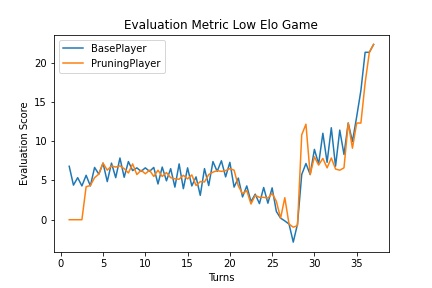
\includegraphics[scale= 0.38]{low_game_eval.jpg}
    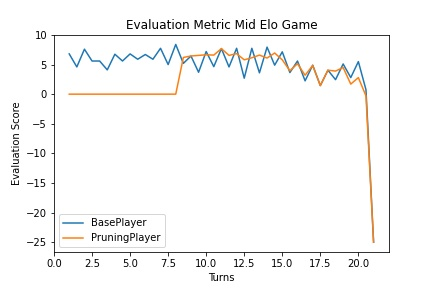
\includegraphics[scale= 0.38]{mid_game_eval.jpg}
    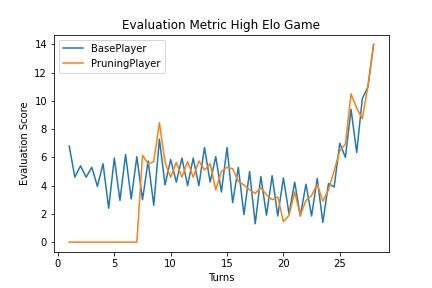
\includegraphics[scale= 0.38]{high_game_eval.jpg}

    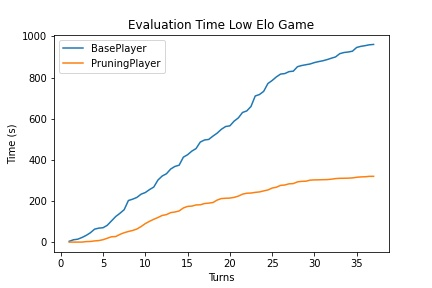
\includegraphics[scale= 0.38]{low_game_time.jpg}
    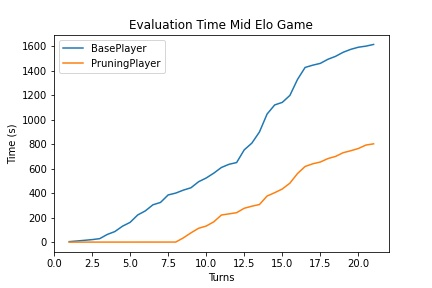
\includegraphics[scale= 0.38]{mid_game_time.jpg}
    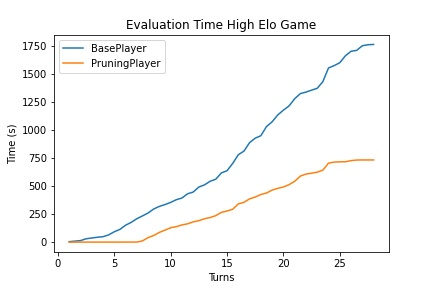
\includegraphics[scale= 0.38]{high_game_time.jpg}
  
    \caption{Comparison made between RulePlayer and PruningPlayer. \newline Top side shows the evaluation scores determined by the Players. Note the smoother evaluation scores made by PruningPlayer on all three of the games. \newline Bottom side shows the cumulative runtime of these Players. Note the flat lines on the Mid Elo and High Elo, indicating the Case-based retrieval at work.} 
\end{figure*}

\begin{figure*}
    \center

    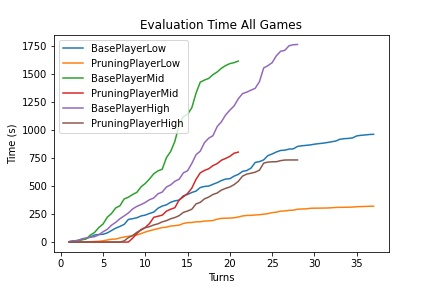
\includegraphics[scale = 0.9]{all_game_time.jpg}
  
    \caption{Comparison of evaluation time in all the three games.} 
\end{figure*}
\section{Conclusions and Future Work}
This research presents project work performed to investigate \acrshort{cbr}-based opening strategy, heuristic tuning, rule-based pruning, and positional evaluation in chess.  In this project, Josep Han focused on evaluation, along with detailwork and tuning of the minimax algorithm, Rowan Lavelle focused on the minimax algorithm and weight testing for the heuristic, and Zach Wilkerson focused on pruning and object-oriented work for the minimax algorithm.  Each author presents the model and results information corresponding to their specialty section, and Rowan spearheads the introduction, Zach the related work, and Josep the conclusions and future work.

\end{document}
